\documentclass[main.tex]{subfiles}
\pagestyle{assignment}

\usepackage{tikz}
\usepackage{subcaption}

\begin{document}
\setcounter{chapter}{26}
\chapter{Assignment}
\label{ch:assignment1}
\thispagestyle{assignment}


\begin{homework}
    [Amazon valley metric]
    Define the metric on $\mathbb{R}^2$ as follows: 
    \begin{equation}
        d((x, y), (x', y')) = 
        \begin{cases}
            |y - y'|, & \text{if } x = x'\\
            |y| + |x - x'| + |y'|, & \text{otherwise}
        \end{cases}
    \end{equation}
    \begin{enumerate}
        \item[(a)] Show that this is indeed a metric. 
        \item[(b)] Draw a ball of radius $1$ centered at $(0, 0)$; a ball of radius $0.5$ centered at $(0, 1)$; a ball of radius $1.5$ centered at $(0, 1)$. 
        \item[(c)] Is $\mathbb{R}^2$ with this metric connected? 
        \item[(d)] Is it first countable? 
        \item[(e)] Is it second bountable? 
        \item[(f)] Is it complete? 
        \item[(g)] Is the unit square $[0, 1] \times [0, 1]$ bounded with respect to $d$? If yes, find its diameter. 
        \item[(h)] Is the unit square $[0, 1] \times [0, 1]$ compact in the topology given by $d$?
        \item[(i)] A function $f: \mathbb{R}^2 \rightarrow \mathbb{R}$ is continuous in the usual sense (in the standard Euclidean topology). Is it always true that $f$ is continuous on $\mathbb{R}^2$ with the topology given by the metric $d$? 
        \item[(j)] A function $g: \mathbb{R}^2 \rightarrow \mathbb{R}$ is continuous in the topology given by $d$. Is it always true that $g$ is continuous in the Euclidean topology?         
    \end{enumerate}
\end{homework}
\par \noindent \textbf{Solution to (a)}
\par We need to verify the four properties of a metric:
\begin{itemize}
    \item Non-negativity: For any $(x, y), (x', y') \in \mathbb{R}^2$, we have $d((x, y), (x', y')) \geq 0$ since it is defined as the sum of absolute values.
    \item Identity of indiscernibles: $d((x, y), (x', y')) = 0$ if and only if $(x, y) = (x', y')$. 
    \par One direction is clear: if $(x, y) = (x', y')$, then $d((x, y), (x', y')) = |y - y'| = 0$. 
    \par For the other direction, suppose $d((x, y), (x', y')) = 0$. If $x = x'$, then $|y - y'| = 0$, so $y = y'$. If $x \neq x'$, then $d((x, y), (x', y')) = |y| + |x - x'| + |y'| = 0$ implies that $|y| = 0$, $|x - x'| = 0$, and $|y'| = 0$, which means $y = 0$, $x = x'$, and $y' = 0$. Thus, $(x, y) = (x', y')$. 
    \item Symmetry: For any $(x, y), (x', y') \in \mathbb{R}^2$, we have $d((x, y), (x', y')) = d((x', y'), (x, y))$. This follows directly from the definition of $d$.
    \item Triangle inequality: For any $(x, y), (x', y'), (x'', y'') \in \mathbb{R}^2$, we need to show that 
    \begin{equation}
        d((x, y), (x'', y'')) \leq d((x, y), (x', y')) + d((x', y'), (x'', y''))
    \end{equation}
    There are four cases based on the values of $x, x', x''$:
    \begin{enumerate}
        \item Case 1: $x = x' = x''$. In this case, we have
        \begin{equation}
            d((x, y), (x'', y'')) = |y - y''| \leq |y - y'| + |y' - y''| = d((x, y), (x', y')) + d((x', y'), (x'', y''))
        \end{equation}
        \item Case 2: $x = x'' \neq x'$. In this case, we have
        \begin{equation}
            \begin{split}
                d((x, y), (x'', y'')) & = |y - y''| \\
                & \leq |y| + |y''| \\
                & \le |y| + |x - x'| + |y'| + |y'| + |x' - x''| + |y''|\\
                & = d((x, y), (x', y')) + d((x', y'), (x'', y''))
            \end{split}
        \end{equation}
        \item Case 3: $x' = x'' \neq x$. In this case, we have
        \begin{equation}
            \begin{split}
                d((x, y), (x'', y'')) & = |y| + |x - x''| + |y''|\\
            & = |y| + |x - x'| + |y''|\\
            & \leq |y| + |y'| + |y''-y'| + |x - x'| \\
            & = d((x, y), (x', y')) + d((x', y'), (x'', y''))
            \end{split}
        \end{equation}
        \item Case 4: $x, x', x''$ are all distinct. In this case, we have
        \begin{equation}
            \begin{split}
                d((x, y), (x'', y'')) & = |y| + |x - x''| + |y''| \\
                & \leq |y| + |x - x'| + |x' - x''| + |y''| + 2|y'|\\
                & = d((x, y), (x', y')) + d((x', y'), (x'', y''))
            \end{split}
        \end{equation}
    \end{enumerate}
    For all cases, the triangle inequality holds. 
\end{itemize}
\par \noindent \textbf{Solution to (b)} 
\begin{figure}[h!]
            \centering
            \begin{subfigure}[b]{0.3\textwidth}
                \centering
                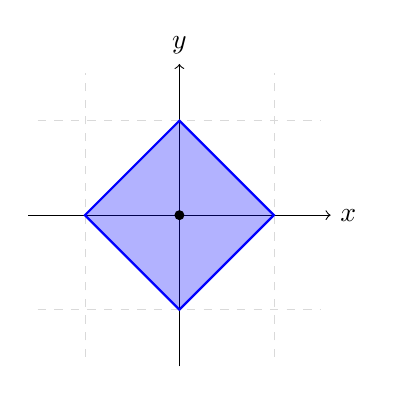
\begin{tikzpicture}[scale=1.2]
                    \draw[help lines, color=gray!30, dashed] (-1.5,-1.5) grid (1.5,1.5);
                    \draw[->] (-1.6,0) -- (1.6,0) node[right] {$x$};
                    \draw[->] (0,-1.6) -- (0,1.6) node[above] {$y$};
                    % Ball 1: Center (0,0), r=1. Shape: |x|+|y|<1
                    \fill[blue, opacity=0.3] (0,1) -- (1,0) -- (0,-1) -- (-1,0) -- cycle;
                    \draw[blue, thick] (0,1) -- (1,0) -- (0,-1) -- (-1,0) -- cycle;
                    \fill[black] (0,0) circle (1.5pt);
                \end{tikzpicture}
                \caption{$B((0,0), 1)$}
            \end{subfigure}
            \hfill
            \begin{subfigure}[b]{0.3\textwidth}
                \centering
                \begin{tikzpicture}[scale=1.2]
                    \draw[help lines, color=gray!30, dashed] (-1,-0.5) grid (1,2);
                    \draw[->] (-1.2,0) -- (1.2,0) node[right] {$x$};
                    \draw[->] (0,-0.6) -- (0,2.2) node[above] {$y$};
                    % Ball 2: Center (0,1), r=0.5. Shape: line segment on x=0
                    \draw[red, line width=2.5pt] (0, 0.5) -- (0, 1.5);
                    \fill[black] (0,1) circle (1.5pt);
                \end{tikzpicture}
                \caption{$B((0,1), 0.5)$}
            \end{subfigure}
            \hfill
            \begin{subfigure}[b]{0.3\textwidth}
                \centering
                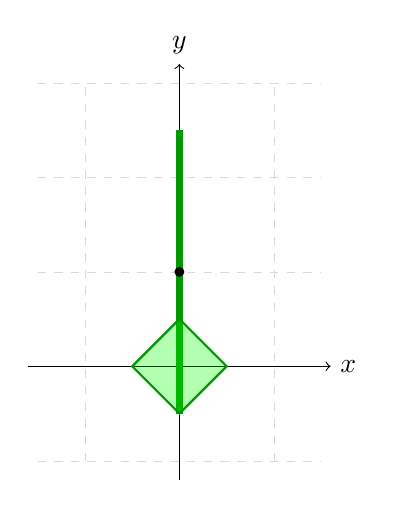
\begin{tikzpicture}[scale=1.2]
                    \draw[help lines, color=gray!30, dashed] (-1.5,-1) grid (1.5,3);
                    \draw[->] (-1.6,0) -- (1.6,0) node[right] {$x$};
                    \draw[->] (0,-1.2) -- (0,3.2) node[above] {$y$};
                    % Ball 3: Center (0,1), r=1.5. Shape: segment on x=0 + diamond near origin
                    \draw[green!60!black, line width=2.5pt] (0, -0.5) -- (0, 2.5);
                    \fill[green, opacity=0.3] (0,0.5) -- (0.5,0) -- (0,-0.5) -- (-0.5,0) -- cycle;
                    \draw[green!60!black, thick] (0,0.5) -- (0.5,0) -- (0,-0.5) -- (-0.5,0) -- cycle;
                    \fill[black] (0,1) circle (1.5pt);
                \end{tikzpicture}
                \caption{$B((0,1), 1.5)$}
            \end{subfigure}
            \caption{Balls in the Amazon valley metric}
        \end{figure}

\par \noindent \textbf{Solution to (c)}
\par Yes. We can show that any two points in $\mathbb{R}^2$ can be connected by a path. Given two points $(x_1, y_1)$ and $(x_2, y_2)$. 
\begin{enumerate}
    \item If $x_1 = x_2$, we can connect them by the vertical line segment between them: $\gamma(t) = (x_1, (1-t)y_1 + ty_2)$ for $t \in [0, 1]$. Then $d(\gamma(t), \gamma(t')) = |(1-t)y_1 + ty_2 - ((1-t')y_1 + t'y_2)| = |(t' - t)(y_1 - y_2)|$. Then for $\epsilon > 0$, choose $\delta = \frac{\epsilon}{|y_1 - y_2|}$, we have $d(\gamma(t), \gamma(t')) < \epsilon$ whenever $|t - t'| < \delta$. Thus, $\gamma$ is continuous. 
    \item Suppose $x_1 \neq x_2$. Without loss of genelarity, let $y_1 \ge 0$, $y_2 \ge 0$ and $x_1 < x_2$. We can connect them by a two-segment path: first move vertically from $(x_1, y_1)$ to $(x_1, 0)$, then move horizontally from $(x_1, 0)$ to $(x_2, 0)$, and finally move vertically from $(x_2, 0)$ to $(x_2, y_2)$. Let $l_1 + l_2 + l_3 = L$. Define the path $\gamma: [0, 1] \rightarrow \mathbb{R}^2$ as follows:
    \begin{equation}
        \gamma(t) = 
        \begin{cases}
            (x_1, y_1 - Lt), & 0 \leq t \leq \frac{y_1}{L} \\
            (x_1 + L(t - \frac{y_1}{L}), 0), & \frac{y_1}{L} \leq t \leq \frac{y_1 + x_2 - x_1}{L} \\
            (x_2, 0 + L(t - \frac{y_1 + x_2 - x_1}{L})), & \frac{y_1 + x_2 - x_1}{L} \leq t \leq 1
        \end{cases}
    \end{equation}
    \par If $\gamma(t), \gamma(t')$ are in the same segment, we can show continuity similarly as in case 1. 
    \par If $\gamma(t)$ is in the vertical segment and $\gamma(t')$ is in the horizontal segment, then $0\le t \le \frac{y_1}{L}$ and $ \frac{y_1}{L} \leq t' \leq \frac{y_1 + x_2 - x_1}{L}$. Without loss of generality, assume $t < t'$. Then for any $\epsilon > 0$, choose $\delta = \frac{\epsilon}{2L}$. If $|t - t'| < \delta$, then 
    \begin{equation}
         \begin{split}
            d(\gamma(t), \gamma(t')) & = |y_1 - Lt| + |x_1 + L(t' - \frac{y_1}{L}) - x_1| \\
            & = |y_1 - Lt| + |Lt' - y_1| \\
            & = y_1 - Lt + Lt' - y_1 \\
            & = L(t' - t) < L \cdot \frac{\epsilon}{2L} = \frac{\epsilon}{2} < \epsilon
         \end{split}
    \end{equation}
    \par Suppose $\gamma(t)$ and $\gamma(t')$ are in different vertical segments, then $0 \le t \le \frac{y_1}{L}$ and $\frac{y_1 + x_2 - x_1}{L} \leq t' \leq 1$. Without loss of generality, assume $t < t'$, $y_1 \ge 0, y_2 \ge 0$ and $x_1 < x_2$. Then for any $\epsilon > 0$, choose $\delta = \frac{\epsilon}{2L}$. If $|t - t'| < \delta$, then
    \begin{equation}
         \begin{split}
            d(\gamma(t), \gamma(t')) & = |y_1 - Lt| + |x_2 - x_1| + |0 + L(t' - \frac{y_1 + x_2 - x_1}{L})| \\
            & = L(t' - t)\\
            & < L \cdot \frac{\epsilon}{2L} = \frac{\epsilon}{2} < \epsilon
         \end{split}
    \end{equation}
\end{enumerate}
Hence, $\gamma$ is continuous and connects $(x_1, y_1)$ and $(x_2, y_2)$. Therefore, $\mathbb{R}^2$ with this metric is path-connected, and thus connected. 
\par \noindent \textbf{Solution to (d)} 
\par Yes. We know from the lectures that every metric space is first countable.  
\par \noindent \textbf{Solution to (e)} 
\par No. Consider the collection of open balls $\{B((x, 1), 1) : x \in \mathbb{R}\}$. We know from (b) that it is like a vertical line segment of length $2$ centered at $(x, 1)$. Then we have uncountably many disjoint open sets. Thus, there cannot be a countable basis. 
\par \noindent \textbf{Solution to (f)}
\par Yes. 
\par Suppose we have a Cauchy sequence $\{(x_n, y_n)\}$ in $\mathbb{R}^2$ with respect to the metric $d$. Then we have two cases:
\begin{enumerate}
    \item For sufficiently large $N$, $x_n = x_m$ for all $n, m \geq N$. In this case, $\{y_n\}$ is a Cauchy sequence in $\mathbb{R}$ with the usual metric. Since $\mathbb{R}$ is complete, there exists $y \in \mathbb{R}$ such that $y_n \rightarrow y$ as $n \rightarrow \infty$. Thus, the sequence $\{(x_n, y_n)\}$ converges to $(x_N, y)$ in $\mathbb{R}^2$ with respect to the metric $d$. 
    \item For any $N$, there exist $n, m \geq N$ such that $x_n \neq x_m$. In this case, for any $\epsilon > 0$, there exists $M \ge N$ such that for all $n, m \geq M$, we have 
    \begin{equation}
        d((x_n, y_n), (x_m, y_m)) = |y_n| + |x_n - x_m| + |y_m| < \epsilon 
    \end{equation}
    This implies that $|y_n| < \epsilon$ and $|y_m| < \epsilon$ for all $n, m \geq M$. Thus, $y_n \rightarrow 0$ as $n \rightarrow \infty$. 
    And this also implies that $|x_n - x_m| < \epsilon$ for all $n, m \geq M$. Thus, $\{x_n\}$ is a Cauchy sequence in $\mathbb{R}$ with the usual metric. Since $\mathbb{R}$ is complete, there exists $x \in \mathbb{R}$ such that $x_n \rightarrow x$ as $n \rightarrow \infty$. Thus, the sequence $\{(x_n, y_n)\}$ converges to $(x, 0)$ in $\mathbb{R}^2$ with respect to the metric $d$. 
\end{enumerate} 
\par \noindent \textbf{Solution to g} 
\par Yes. For any two points $(x_1, y_1), (x_2, y_2) \in [0, 1] \times [0, 1]$, we have 
\begin{equation}
    d((x_1, y_1), (x_2, y_2)) \leq |y_1| + |x_1 - x_2| + |y_2| \leq 1 + 1 + 1 = 3 
\end{equation}
Thus, the diameter of the unit square is at least $3$. 
And for $(0, 1), (1, 1) \in [0, 1] \times [0, 1]$, we have
\begin{equation}
    d((0, 1), (1, 1)) = |1| + |0 - 1| + |1| = 3
\end{equation}
Thus, the diameter of the unit square is exactly $3$.
\par \noindent \textbf{Solution to h}
\par We can first cover the $\frac{3}{4}$ of the unit square by $B((0, 0), 1)$ and $B((1, 0), 1)$(whose shapes are similar to the first figure of (b)). 
\par And we can cover the remaining area by infinitely many vertical segments like $B((x, 1), 0.5)$ for $x \in [0, 1]$(whose shapes are similar to the second figure of (b)).  
\par The problem is we can't pick finitely many of these vertical segments to cover the top edge of the unit square. Each point on the top edge $(x, 1)$ can only be covered by $B((x, 1), 0.5)$ thus we need uncountably many of them to cover the whole top edge. 
\par Thus, the unit square $[0, 1] \times [0, 1]$ is not compact in the topology given by $d$.

\par \noindent \textbf{Solution to i} 
\par Yes. The topology on $\mathbb{R}$ is not specified, so we assume it is the usual topology. 
\par First we can see that the Euclidean topology on $\mathbb{R}^2$ is coarser than the topology given by the metric $d$. We know that the collection of open balls in the Euclidean metric forms a basis for the Euclidean topology. For any open ball $B_e((x, y), r)$ in the Euclidean metric, we can find an open ball $B_d((x, y), r)$ in the metric $d$ such that $B_d((x, y), r) \subseteq B_e((x, y), r)$. Thus, every open set in the Euclidean topology is also an open set in the topology given by the metric $d$. 
\par We know that a function $f: \mathbb{R}^2 \rightarrow \mathbb{R}$ is continuous if the preimage of every open set in $\mathbb{R}$ is an open set in $\mathbb{R}^2$. Now we have an open set $U \subseteq \mathbb{R}$. Then we have $f^{-1}(U)$ is an open set in the Euclidean topology on $\mathbb{R}^2$. Since the Euclidean topology is coarser than the topology given by the metric $d$, $f^{-1}(U)$ is also an open set in the topology given by the metric $d$. Thus, $f$ is continuous on $\mathbb{R}^2$ with the topology given by the metric $d$.

\par \noindent \textbf{Solution to j} 
\par No. 
\par We define $g: \mathbb{R}^2 \rightarrow \mathbb{R}$ by 
\begin{equation}
    g(x, y) = 
    \begin{cases}
        y, & \text{if } x = 0\\
        0, & \text{otherwise}
    \end{cases}
\end{equation}
\par It is enough to show that the preimage of a basis in $\mathbb{R}$ is open in $\mathbb{R}^2$ with the topology given by the metric $d$. Consider a basis element $(a, b) \subseteq \mathbb{R}$. 
\par If $0 \notin (a, b)$, then $g^{-1}((a, b)) = \{(0, y)| y\in (a, b)\}$ which is open in the topology given by the metric $d$. 
\par If $0 \in (a, b)$, then $g^{-1}((a, b)) = \{(x, y)| x\neq 0\}$ which can be the union of three types of open sets:
\begin{enumerate}
    \item $B((x, 0), r)$ for any $x \neq 0$ and $0 < r < \min(|a|, |b|)$; 
    \item $B((0, y), r)$ for any $y \in (a, b)$ and $r < \min\{|y - a|, |y - b|\}$; 
    \item $B((x, y), \frac{|y|}{2})$ for any $x \neq 0$, $y > 0$. 
\end{enumerate}
\mbox{} \\ \null \hfill $\blacksquare$ 
 


\begin{homework}
    Let $X = \mathbb{R}^2$. Show that the one-point compactification of $X$ is homeomorphic to the sphere $S^2 = \{(x, y, z) \in \mathbb{R}^3 : x^2 + y^2 + z^2 = 1\}$. 
\end{homework}
\par \noindent \textbf{Solution} 
\par The one-point compactification of $X$ is $\hat{X} = X \cup \{\infty\}$ where $\infty$ is a point not in $X$. 
\par The topology on $\hat{X}$ is defined as follows: 
\begin{itemize}
    \item For any open set $U \subseteq X$, $U$ is also an open set in $\hat{X}$. 
    \item For any open set $U \subseteq \hat{X}$ that contains $\infty$, its complement $\hat{X} \setminus U$ is a compact subset of $X$. 
\end{itemize}
\par We have verify in the lectures that the topology on $\hat{X}$ is indeed a topology. 
\par We define a map $f: \hat{X} \rightarrow S^2$ as follows:
\begin{equation}
    f(p) = 
    \begin{cases}
        \left(\frac{2x}{x^2 + y^2 + 1}, \frac{2y}{x^2 + y^2 + 1}, \frac{x^2 + y^2 - 1}{x^2 + y^2 + 1}\right), & p = (x, y) \in X\\
        (0, 0, 1), & p = \infty
    \end{cases}
\end{equation}
\par It is easy to check that $f$ is a bijection and the restriction of $f$ on $X$ is a homeomorphism between $X$ and $S^2 \setminus \{(0, 0, 1)\}$. 
\par Next, we show that $f$ is continuous. 
\par For any open set $U \subseteq S^2$ that does not contain the north pole $(0, 0, 1)$, we have $f^{-1}(U)$ is an open set in $X$ since the restriction of $f$ on $X$ is continuous. 
\par For any open set $U \subseteq S^2$ that contains the north pole $(0, 0, 1)$, its complement $S^2 \setminus U$ is a closed subset of $S^2$ that does not contain the north pole. Thus, $f^{-1}(S^2 \setminus U)$ is a closed subset of $X$. Since $S^2 \setminus U$ is compact, $f^{-1}(S^2 \setminus U)$ is also compact. Thus, $f^{-1}(U) = \hat{X} \setminus f^{-1}(S^2 \setminus U)$ is an open set in $\hat{X}$. 
\par Next, we show that $f^{-1}$ is continuous. 
\par For any open set $V \subseteq \hat{X}$ that does not contain $\infty$, we have $f(V)$ is an open set in $S^2$ since the restriction of $f^{-1}$ on $S^2 \setminus \{(0, 0, 1)\}$ is continuous. 
\par For any open set $V \subseteq \hat{X}$ that contains $\infty$, its complement $\hat{X} \setminus V$ is a compact subset of $X$. Thus, $f(\hat{X} \setminus V)$ is a compact subset of $S^2$ that does not contain the north pole thus is closed. Thus, $f(V) = S^2 \setminus f(\hat{X} \setminus V)$ is an open set in $S^2$. 
\par Therefore, $f$ is a homeomorphism between $\hat{X}$ and $S^2$.
\mbox{} \\ \null \hfill $\blacksquare$ 

\begin{homework}
    Let $\mathbb{C}$ be equipped with the co-countable topology: a set $U \subseteq \mathbb{C}$ is open if and only if its complement $\mathbb{C}\setminus U$ is at most countable. 
    \begin{enumerate}
        \item [(a)] Prove that every polynomial function $f: \mathbb{C} \rightarrow \mathbb{C}$ is continuous in this topology. 
        \item [(b)] Is it true that every function $f: \mathbb{C} \rightarrow \mathbb{C}$ that is continuous in this topology is a polynomial? Justify your answer.
    \end{enumerate}
\end{homework}

\par \noindent \textbf{Solution to (a)} 
\par Let $f: \mathbb{C} \rightarrow \mathbb{C}$ be a polynomial function. We need to show that for any open set $U \subseteq \mathbb{C}$ in the co-countable topology, $f^{-1}(U)$ is also an open set in the co-countable topology. 
\par Let $U \subseteq \mathbb{C}$ be an open set in the co-countable topology(The case for $U = \emptyset$ or $\mathbb{C}$ is trivial). Then its complement $\mathbb{C} \setminus U$ is at most countable. Then we have 
\begin{equation}
    f^{-1}(U) = f^{-1}(\mathbb{C} \setminus (\mathbb{C} \setminus U)) = \mathbb{C} \setminus f^{-1}(\mathbb{C} \setminus U)
\end{equation}
So it suffices to show that any preimage of a countable set under $f$ is also countable. 
\par Let $A \subseteq \mathbb{C}$ be a countable set, i.e., $A = \{a_1, a_2, \ldots\}$. By the Fundamental Theorem of Algebra, for each $a_i$, the equation $f(z) = a_i$ has at most $\deg(f)$ solutions. Thus, we have 
\begin{equation}
    f^{-1}(A) = \bigcup_{i\in \mathbb{N}} f^{-1}(\{a_i\})
\end{equation}
is a countable union of finite sets, which is countable. 
\par \noindent \textbf{Solution to (b)} 
\par Let $f: \mathbb{C} \rightarrow \mathbb{C}$ be defined by $f(z) = e^z$. $f$ is not a polynomial function. We show that $f$ is continuous in the co-countable topology. 
\par Let $A \subseteq \mathbb{C}$ be a countable set, i.e., $A = \{a_1, a_2, \ldots\}$. Let $a_i = r e^{i\theta}$ in polar form. Then the equation $e^z = a_i$ has solutions $z = \ln r + i(\theta + 2k\pi)$ for all $k \in \mathbb{Z}$. Thus, we have
\begin{equation}
    f^{-1}(A) = \bigcup_{i\in \mathbb{N}} f^{-1}(\{a_i\}) = \bigcup_{i\in \mathbb{N}} \{\ln r + i(\theta + 2k\pi) : k \in \mathbb{Z}\} 
\end{equation}
is a countable union of countable sets, which is countable. Thus, $f$ is continuous in the co-countable topology. 
\mbox{} \\ \null \hfill $\blacksquare$ 

\begin{homework}
    Consider the space $\{0, 1\}^{\omega}$ (the space of maps $\mathbb{N} \rightarrow \{0, 1\}$) with the product topology. 
    \begin{enumerate}
        \item [(a)] Is this space compact? 
        \item [(b)] Is it metrizable? 
        \item [(c)] Is the subspace consisting of sequences with finitely many $1$'s compact? 
    \end{enumerate}
\end{homework}

\par \noindent \textbf{Solution to (a)}
\par It is not specified. But we let the topology on $\{0, 1\}$ be the discrete topology by default.  
\par Yes. By Tychonoff's theorem, the product of compact spaces is compact. Since $\{0, 1\}$ with the discrete topology is a finite set and thus compact, $\{0, 1\}^{\omega}$ with the product topology is compact.
\par \noindent \textbf{Solution to (b)} 
\begin{theorem}
    The space $\mathbb{R}^{\omega}$ with the product topology is metrizable.
\end{theorem}
\par We've given the proof of this theorem in the lectures. 
\par We can let $d$ be any metric on $\mathbb{R}^{\omega}$ that induces the product topology. Then we can restrict $d$ on the subspace $\{0, 1\}^{\omega}$. Thus, $\{0, 1\}^{\omega}$ with the product topology is metrizable because it is a subspace of a metrizable space. 
\par \noindent \textbf{Solution to (c)}  
\par No. 
\par The space $\{0, 1\}$ with the discrete topology is Hausdorff. 

\begin{theorem}
    The product of Hausdorff spaces is Hausdorff. 
\end{theorem}
\begin{theorem}
    A compact subspace of a Hausdorff space is closed.
\end{theorem}

\par By the two theorems above, we know that $\{0, 1\}^{\omega}$ with the product topology is Hausdorff. 

\par We prove by contrary that the subspace $Y$ consisting of sequences with finitely many $1$'s is not compact. 
\par Assume $Y$ is compact then by the above theorems $Y$ is closed in $\{0, 1\}^{\omega}$. 
\par We define a sequence $\{x_n\}$ in $Y$ as follows: 
\begin{equation}
    x_n = (\underbrace{1, 1, \ldots, 1}_{n\text{ times}}, 0, 0, 0, \ldots)
\end{equation}
\par It is easy to see that $x_n \rightarrow x = (1, 1, 1, \ldots)$ in $\{0, 1\}^{\omega}$ with the product topology. Since $Y$ is closed, we have $x \in Y$. But this is a contradiction because $x$ has infinitely many $1$'s. 
\mbox{} \\ \null \hfill $\blacksquare$ 

\begin{homework}
    Let $X$ be a compact Hausdorff space. 
    \begin{enumerate}
        \item [(a)] Show that $X$ is normal. 
        \item [(b)] Prove that if $X$ has a countable basis, then it is metrizable. 
        \item [(c)] Give an example showing that compactness cannot be omitted. 
    \end{enumerate}
\end{homework}

\par \noindent \textbf{Solution to (a)} 
\par Hausdorffness($T_2$) implies that $X$ is $T_1$.  
\par First we'll show that $X$ is regular. Take $x \in X$ and a closed set $F \subseteq X$ such that $x \notin F$. For each $y \in F$, by Hausdorffness, there exist disjoint open sets $U_y$ and $V_y$ such that $x \in U_y$ and $y \in V_y$. Then $\{V_y : y \in F\}$ is an open cover of $F$. Since $F$ is closed in a compact space, $F$ is compact. Thus, there exists a finite subcover $\{V_{y_1}, V_{y_2}, \ldots, V_{y_n}\}$. Let $U = \bigcap_{i=1}^n U_{y_i}$ and $V = \bigcup_{i=1}^n V_{y_i}$. Then $U$ and $V$ are disjoint open sets such that $x \in U$ and $F \subseteq V$. Thus, $X$ is regular. 

\par Second we will show that $X$ is normal. Take two disjoint closed sets $A, B \subseteq X$. For each $a \in A$, by regularity, there exist disjoint open sets $U_a$ and $V_a$ such that $a \in U_a$ and $B \subseteq V_a$. Then $\{U_a : a \in A\}$ is an open cover of $A$. Since $A$ is closed in a compact space, $A$ is compact. Thus, there exists a finite subcover $\{U_{a_1}, U_{a_2}, \ldots, U_{a_m}\}$. Let $U = \bigcup_{i=1}^m U_{a_i}$ and $V = \bigcap_{i=1}^m V_{a_i}$. Then $U$ and $V$ are disjoint open sets such that $A \subseteq U$ and $B \subseteq V$. Thus, $X$ is normal.

\par \noindent \textbf{Solution to (b)}

\begin{theorem}
    A topological space $X$ is metrizable if and only if $X$ is second-countable, regular($T_3$) and $T_1$.
\end{theorem}
\par We've given the proof of this theorem in the lectures. 
\par From (a), we know that $X$ is normal thus regular. And since $X$ is Hausdorff, it is $T_1$. And we are given that $X$ has a countable basis, i.e., $X$ is second-countable. Thus, by the theorem above, $X$ is metrizable. 
\par \noindent \textbf{Solution to (c)}
\par Consider the $K$ topology on $\mathbb{R}$. Let $K = \{1/n : n \in \mathbb{N}\}$. The $K$-topology on $\mathbb{R}$ is defined as follows: a set $U \subseteq \mathbb{R}$ is open if and only if it is of the form 
\begin{itemize}
    \item [(i)] $U$ is an open set in the usual topology on $\mathbb{R}$; or 
    \item [(ii)] $U$ is of the form $V \setminus K$ where $V$ is an open set in the usual topology on $\mathbb{R}$.
\end{itemize} 
\par It is easy to check that the $K$-topology on $\mathbb{R}$ is indeed a topology. 
\par It is Hausdorff because $K$-topology is finer than the usual topology on $\mathbb{R}$ and the usual topology on $\mathbb{R}$ is Hausdorff. 
\par It has a countable basis we can consider $B_r(q)$ for all rational numbers $q$ and rational numbers $r > 0$ and $B_r(q) \setminus K$ for all rational numbers $q$ and rational numbers $r > 0$. 
\par It is not compact. Consider the open cover $\mathcal{U} = \{(-n, n)\setminus K : n \in \mathbb{N}\}$. Any finite subcover of $\mathcal{U}$ has a largest interval $(-N, N)\setminus K$ for some $N \in \mathbb{N}$. But then $N+1 \notin (-N, N)\setminus K$. Thus, $\mathcal{U}$ has no finite subcover. 
\par It is not metrizable. By the Urysohn's metrization theorem, it is enough to show that $X$ is not regular. 
\par Consider the point $x = 0$ and the closed set $F = K$. For each open set $U$ containing $x$, there are two cases: 

\begin{enumerate}
    \item If $U$ is an open set in the usual topology on $\mathbb{R}$, then there exists $N \in \mathbb{N}$ such that $1/N \in U$. Thus, any open set $V$ containing $F$ must intersect with $U$ because $1/N \in F \cap U$. 
    \item If $U$ is of the form $V \setminus K$ where $V$ is an open set in the usual topology on $\mathbb{R}$. Then there exists $\epsilon'$ such that $0\in (-\epsilon', \epsilon') \subseteq V$. And $U' $ is an open set containing $F$. Then $U'$ is the open set in the usual topology. But $U'$ must contains $1/N$ for all $N \in \mathbb{N}$. Then there exists $\epsilon > 0$ such that $(0, \epsilon) \subseteq U'$. Thus $(0, \min(\epsilon, \epsilon')) \subseteq U \cap U' \neq \emptyset$. 
\end{enumerate}
\mbox{} \\ \null \hfill $\blacksquare$ 

\end{document}